\chapter{微分方程速成}\label{app:de}

微分方程（DE）是对动态系统进行建模的基本工具，大体上可以分为\emph{常微分方程}（ODE）、\emph{随机微分方程}（SDE）和\emph{偏微分方程}（PDE）三类。

常微分方程描述了一个系统的状态如何按照某种精确的规则随时间变化，因此只要知道起点，就能完全确定其未来的轨迹。随机微分方程在这种演化过程中引入了随机性，用以刻画噪声或不确定性对系统行为的影响，使得结果不再是确定性的，而是具有概率性质。偏微分方程则解释了依赖于多个变量（例如时间和空间）的函数如何共同演化，能够描述诸如热量扩散、波动传播，以及\emph{随机系统中概率密度的时间演化}等现象（剧透：Fokker-Planck 方程）。这些类型的微分方程构成了一种基础语言，用于理解系统在确定性影响与随机性影响下如何随时间和空间演化。

在本章中，我们将介绍微分方程方面的必备预备知识。

\clearpage
\newpage

\section{常微分方程基础}

本节介绍常微分方程的基本理论，着重强调在给定初始条件下解的唯一性。同时，本节还涵盖了使用数值求解器求解常微分方程的实用方法。


\subsection{常微分方程的直观理解}

确定性的过程被称为\emph{常微分方程}（ODE）。在多变量的情形下，我们考虑如下形式的方程组：
\begin{equation}\label{eq:general_ode}
    \frac{\diff \mathbf{x}(t)}{\diff t} = \mathbf{v}(\mathbf{x}(t), t),
\end{equation}
其中 $\mathbf{x}(t) \in \mathbb{R}^D$ 是一个向量值函数，表示系统在时刻 $t$ 的状态；而 $\mathbf{v}: \mathbb{R}^D \times \mathbb{R} \to \mathbb{R}^D$ 是一个向量场，规定了空间和时间内每一点处变化的方向与大小。


\paragraph{求解常微分方程的高层直观。}
\begin{figure}[th]
    \centering
    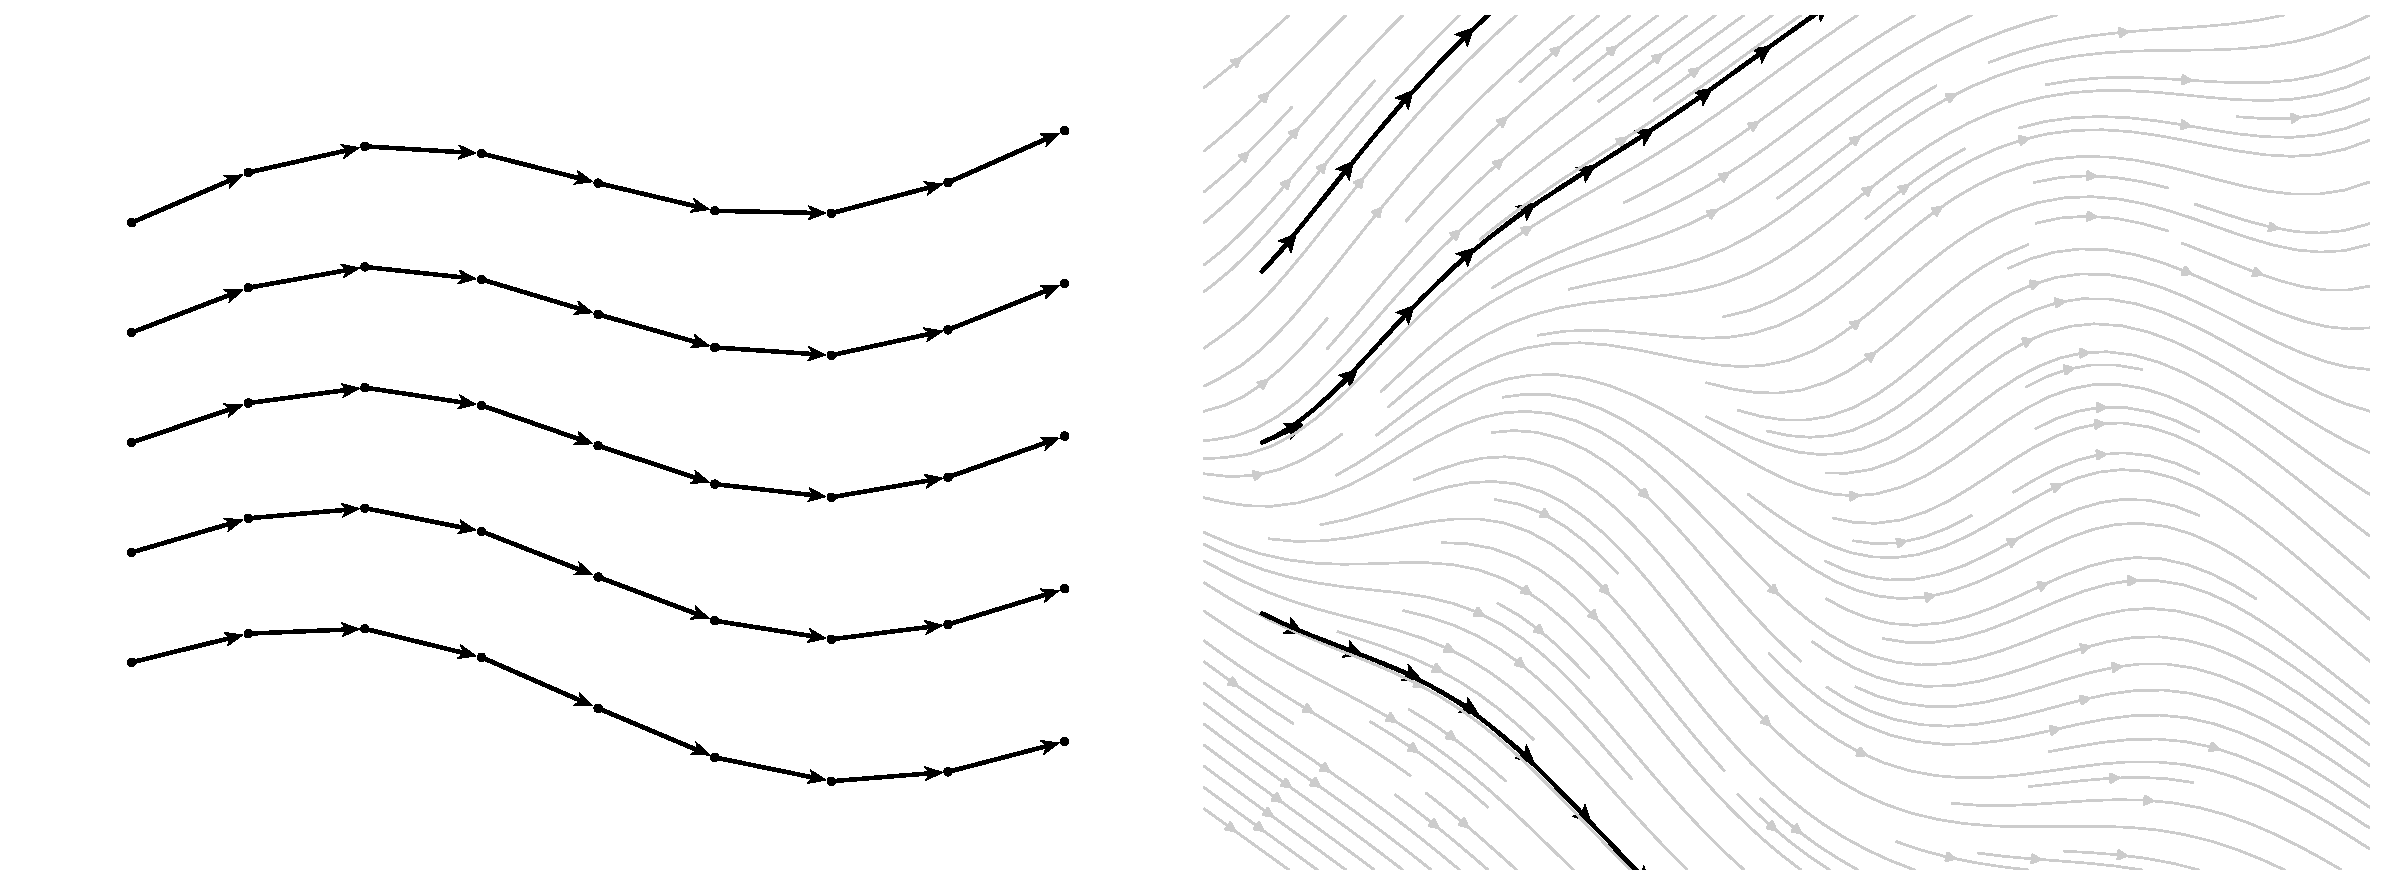
\includegraphics[width=\linewidth]{Images/PartE/discrete_vs_continuous_ode.pdf}
    \caption{\textbfs{常微分方程示意图。}
速度场 $\rvv(\rvx,t)$ 在每一点处都赋予一个漂移向量。
解轨迹 $\rvx(t)$ 是一条路径，其切线方向始终与局部漂移方向一致。
左图展示了逐步推进的求解器更新（点与箭头），用以近似该路径；
右图则展示了与速度场保持一致流动的精确轨迹（黑色）。在未指定初始状态 $\rvx(0)$ 的情况下，存在无穷多条瞬时变化与同一速度场相匹配的轨迹。
然而一旦 $\rvx(0)$ 被固定，常微分方程便唯一确定一条依照漂移方向流动的路径 $\rvx(t)$。
\figcredit{由作者绘制。}}
    \label{fig:ode-illustration}
\end{figure}

为了建立直观理解，可以将向量场 $\mathbf{v}(\mathbf{x}, t)$ 想象成一幅动态的箭头地图，它告诉你一个点 $\mathbf{x}$ 在任意给定时刻 $t$ 应当如何运动。求解这个微分方程，意味着要在这个场中描绘出一条曲线 $\mathbf{x}(t)$，使得该曲线在任一点的切线（即瞬时速度）都与 $\mathbf{v}(\mathbf{x}(t), t)$ 所给出的向量方向一致。
\begin{itemize}
    \item \textbfs{向量场视角：} 函数 $\mathbf{v}(\mathbf{x}, t)$ 定义了事物应当如何运动：它给出了关于运动或变化的局部"指令"。
    \item \textbfs{轨迹视角：} 解 $\mathbf{x}(t)$ 是一条路径，若一个粒子在每一瞬时都遵循由向量场 $\mathbf{v}$ 所设定的规则，它便会沿着这条路径运动。
\end{itemize}
因此，求解一个常微分方程就好比将一个粒子放入流场之中，并观察它随时间的运动方向。

\subsection{常微分方程的存在性与唯一性}
到目前为止，我们已经看到，求解一个常微分方程意味着寻找一条在每一点处都遵循向量场所给方向的路径。直观地讲，这就像是追踪一个粒子沿着由速度所定义的流运动时的轨迹。

但这种图景引出了一个重要的问题：
\begin{question}
    如果我们选定一个起点，能否确信确实存在一条遵循这些方向的路径？如果存在，那么这条路径是唯一的吗，还是粒子有可能突然跳到另一条不同的轨迹上？
\end{question}

回答这些问题至关重要，因为它告诉我们系统的行为能否从其起始位置被可靠地预测。
\emph{存在性与唯一性定理}给出了向量场应满足的条件，这些条件能够保证从任意给定的初始点出发恰好存在一条路径。
这确保了解的行为是一致的，并构成了常微分方程理论的基石。


\paragraph{局部（时间上）的存在性与唯一性定理。}


下面，我们陈述该定理的一个\emph{局部}版本，它断言在给定初始条件下，在初始时刻的某个邻域内解的存在性与唯一性。

\thmp{局部存在性与唯一性}{ode-local}{
设 $\mathbf{v}(\mathbf{x}, t)$ 是关于 $\mathbf{x}$ 和 $t$ 在区域 $D \subseteq \mathbb{R}^D \times \mathbb{R}$ 上的连续函数。如果 $\mathbf{v}$ 关于 $\mathbf{x}$ 满足 Lipschitz 条件：
\[
\|\mathbf{v}(\mathbf{x}_1, t) - \mathbf{v}(\mathbf{x}_2, t)\| \leq L \|\mathbf{x}_1 - \mathbf{x}_2\| \quad \forall (\mathbf{x}_1, t), (\mathbf{x}_2, t) \in D,
\]
其中 $L > 0$ 是常数，那么对于每一个初始条件 $\mathbf{x}(t_0) = \mathbf{x}_0$，都存在唯一的解 $\mathbf{x}(t)$ 在某个区间 $[t_0 - \delta, t_0 + \delta]$ 上满足 \Cref{eq:general_ode}。}{（证明思路）存在性与唯一性定理可以借助 Picard-Lindel\"of 迭代方法进行构造性地证明。该方法生成一个函数序列 $\{\mathbf{x}_n(t)\}$，该序列收敛到解 $\mathbf{x}(t)$。迭代定义为：
\[
\mathbf{x}_{n+1}(t) = \mathbf{x}_0 + \int_{t_0}^t \mathbf{v}(\mathbf{x}_n(s), s) \diff s.
\]
\begin{itemize}
    \item 从一个初始猜测 $\mathbf{x}_0(t) = \mathbf{x}_0$ 出发。
    \item 利用上述积分形式迭代地精化 $\mathbf{x}_n(t)$。
    \item 在 Lipschitz 条件下，通过应用压缩映射原理可保证收敛性。
\end{itemize}
}
该证明的本质根植于 Picard–Lindelöf 迭代方法，其核心思想也在 \Cref{sec:picard} 中被用于加速扩散模型的采样过程。


\paragraph{全局（时间上）的存在性与唯一性定理。}
局部存在性与唯一性定理保证了解在一个小时间区间上的存在性，而"全局（时间上）存在性与唯一性定理"则在附加的正则性条件下将此结果推广到整个区间 $[t_0, T]$。此类中一个著名的结果是 \emph{Carathéodory 定理}，它在两个关键假设下保证常微分方程解的全局存在性与唯一性：状态变量的局部 Lipschitz 连续性，以及线性增长界。

\begin{enumerate}[label=(\roman*)]
    \item \textbfs{关于 $\mathbf{x}$ 的局部 Lipschitz 条件：} 存在一个在 $[0, T]$ 上可积的函数 $\mathrm{Lip}(t)$，使得对所有的 $\mathbf{x}_1, \mathbf{x}_2 \in \mathbb{R}^D$，
    \[
    \|\rvv(\mathbf{x}_1, t) - \rvv(\mathbf{x}_2, t)\| \leq \mathrm{Lip}(t) \|\mathbf{x}_1 - \mathbf{x}_2\|.
    \]

    \item \textbfs{线性增长条件：} 存在一个在 $[0, T]$ 上可积的函数 $M(t)$，使得对所有的 $\mathbf{x} \in \mathbb{R}^D$，
    \[
    \|\rvv(\mathbf{x}, t)\| \leq M(t)(1 + \|\mathbf{x}\|).
    \]
\end{enumerate}
关于这些假设、定理的严格表述及详细证明，我们建议读者参阅 \citep{reid1971ordinary}。

\rmkb{要将这些定理应用于扩散模型中的概率流常微分方程（参见 \Cref{eq:prob_ode_gt}），可能需要对分数函数 $\nabla_\rvx \log p_t(\rvx)$ 施加额外的假设，例如条件 (i) 和 (ii)。对于不关注技术细节的读者而言，这些假设可以合理地直接接受，而无需进一步的论证。
}

总而言之，当给定的初始条件被赋予一个由含时速度场定义的常微分方程时，粒子流动的轨迹便被唯一地确定。

\paragraph{唯一性蕴含解的不相交性} 正如局部存在性与唯一性定理所保证的那样，常微分方程解的唯一性蕴含了一个基本性质：从不同初始条件出发的两条不同的解轨迹不可能相互交叉。这反映了常微分方程的确定性本质，确保每一个状态都沿着一条唯一的路径演化。下面的推论将这一结果形式化。


\corp{解的不相交性}{
考虑常微分方程的两个解 $\rvx_1(t)$ 和 $\rvx_2(t)$
\[
\frac{\diff \rvx(t)}{\diff t} = \rvv\left(\rvx(t),t\right), \quad t \in [0,T].
\]
假设它们具有不同的初始值 $\rvx_1(0) \neq \rvx_2(0)$。那么这两个解在 $[0,T]$ 上不相交，即
\[
\rvx_1(t) \neq \rvx_2(t) \quad \text{for all } t \in [0,T].
\]
}{反证，假设存在某个 $t^* \in (0,T]$ 使得
\[
\mathbf{x}_1(t^*) = \mathbf{x}_2(t^*).
\]
定义两个解首次相遇的时刻为
\[
t_0 := \inf \{ t \in [0,T]|\mathbf{x}_1(t) = \mathbf{x}_2(t) \}.
\]
由于 $\mathbf{x}_1(0) \neq \mathbf{x}_2(0)$ 且 $t^*$ 属于该集合，因此有 $t_0 > 0$。由 $\mathbf{x}_1$ 和 $\mathbf{x}_2$ 的连续性可得
\[
\mathbf{x}_1(t_0) = \mathbf{x}_2(t_0).
\]

考虑初值问题
\[
\frac{\mathrm{d}\mathbf{x}(t)}{\mathrm{d}t} = \mathbf{v}(\mathbf{x}(t), t), \quad \mathbf{x}(t_0) = \mathbf{x}_1(t_0).
\]
由常微分方程的唯一性定理，$\mathbf{x}_1$ 和 $\mathbf{x}_2$ 必须在区间 $[t_0, T]$ 上一致。对时间反向应用唯一性同样意味着这两个解在 $[0, t_0]$ 上也一致。
因此，这两个解满足
\[
\mathbf{x}_1(t) = \mathbf{x}_2(t) \quad \text{for all } t \in [0, T],
\]
这与 $\mathbf{x}_1(0) \neq \mathbf{x}_2(0)$ 的假设相矛盾。由此我们得出结论
\[
\mathbf{x}_1(t) \neq \mathbf{x}_2(t) \quad \text{for all } t \in [0, T].
\]

}

通过保证解的路径不相交，该定理为流映射模型提供了隐含却至关重要的支撑（参见 \Cref{ch:distillation,ch:fast-scratch}）。



\subsection{指数积分因子}\label{app:exp-int-factor}
即使是由一般含时速度 $\rvv$ 所确定的常微分方程也无法得到闭式解，但在某些特殊情形下，我们可以解析地求解它们，或者将其形式归约为一个具有更好结构的形式。
\paragraph{一个示例。}
考虑如下的线性标量常微分方程：
\[
\frac{\diff \rvx(t)}{\diff t} = L(t)\rvx(t),
\]
其中 $L(t) \in \mathbb{R}$ 是连续函数。该方程可求得闭式解，其解广为人知（对任意 $s$ 和 $t$）：
\[
\rvx(t) = \rvx(s) \cdot \exp\left( \int_s^t L(\tau) \,\diff \tau \right).
\]
该公式表明，解是按照一个指数因子演化的，该因子累积了含时系数 $L(t)$ 的效应。这启发我们使用\emph{指数积分因子}：
\begin{align}\label{eq:exp-int-factor}
    \mathcal{E}(s \shortrightarrow t) := \exp\left( \int_s^t L(\tau)\diff \tau \right),
\end{align}
尤其是在动力系统同时包含线性部分和非线性部分的更一般情形下。



\paragraph{半线性常微分方程与指数积分因子。}
现在我们考虑更广泛的一类常微分方程，称为\emph{半线性}常微分方程。这类方程将动力学拆分为（关于状态变量的）线性部分与非线性余项：
\begin{align}\label{eq:semilinear-ode}
    \frac{\diff \rvx(t)}{\diff t} = L(t)\rvx(t) + \rmN(\rvx(t), t),
\end{align}
其中 $\rvx(t) \in \mathbb{R}^D$ 是状态向量，$L(t)$ 是标量值连续函数，$\rmN: \mathbb{R}^D \times [0,T] \to \mathbb{R}^D$ 是非线性向量场。这种半线性结构在许多物理和工程系统中自然地出现。特别地，它也出现在扩散模型的概率流常微分方程表述中（参见 \Cref{eq:prob_ode_gt}）。识别出这种结构使我们能够使用指数积分因子，这不仅简化了分析，还提高了数值稳定性。具体而言，这一技巧在快速扩散常微分方程求解器的设计中扮演了核心角色（参见 \Cref{ch:solvers}）。


\subparagraph{步骤一：通过积分因子分离非线性项。}
观察到我们可以通过从 \Cref{eq:semilinear-ode} 的半线性常微分方程中减去线性漂移项来分离非线性部分：
\[
\frac{\diff \rvx(t)}{\diff t} - L(t)\rvx(t) = \rmN(\rvx(t), t).
\]
为了吸收线性项，我们在等式两边同时乘以积分因子的逆：
\[
\mathcal{E}^{-1}(s \shortrightarrow t) = \exp\left(-\int_s^t L(\tau)\diff \tau \right).
\]
现在对左端应用乘积求导法则：
\begin{align*}
\mathcal{E}^{-1}(s \shortrightarrow t) \left( \frac{\diff \rvx(t)}{\diff t} - L(t)\rvx(t) \right)
&= \frac{\diff}{\diff t} \left[ \mathcal{E}^{-1}(s \shortrightarrow t) \rvx(t) \right].
\end{align*}
因此，方程变为：
\[
\frac{\diff}{\diff t} \left[ \mathcal{E}^{-1}(s \shortrightarrow t) \rvx(t) \right]
= \mathcal{E}^{-1}(s \shortrightarrow t) \rmN(\rvx(t), t).
\]

这一变换通过分离出非线性分量简化了原方程，使我们能够在一个变换后的坐标系中完全专注于非线性动力学。

\subparagraph{步骤二：对时间积分。}
现在我们将等式两边从 $s$ 到 $t$ 积分：
\[
\int_s^t \frac{\diff}{\diff \tau} \left[ \mathcal{E}^{-1}(s \shortrightarrow \tau) \rvx(\tau) \right] \diff \tau
= \int_s^t \mathcal{E}^{-1}(s \shortrightarrow \tau) \rmN(\rvx(\tau), \tau)\diff \tau.
\]
左端就是变换后变量在 $t$ 与 $s$ 处取值之差：
\[
\mathcal{E}^{-1}(s \shortrightarrow t) \rvx(t) - \rvx(s).
\]
于是我们得到：
\[
\mathcal{E}^{-1}(s \shortrightarrow t) \rvx(t)
= \rvx(s) + \int_s^t \mathcal{E}^{-1}(s \shortrightarrow \tau) \rmN(\rvx(\tau), \tau)\diff \tau.
\]

\subparagraph{步骤三：求解 $\rvx(t)$。}
在等式两边同乘指数流 $\mathcal{E}(s \shortrightarrow t)$ 即得解：
\begin{align}\label{eq:exp-int-factor-integration}
    \rvx(t) = \underbrace{\mathcal{E}(s \shortrightarrow t)  \rvx(s)}_{\text{linear part}} + \underbrace{\int_s^t \mathcal{E}(\tau \shortrightarrow t) \rmN(\rvx(\tau), \tau)\diff \tau}_{\text{nonlinear part}} .
\end{align}

解自然地分离为线性分量与非线性分量。指数积分器利用这种结构，以精确的闭式求解线性部分，而仅对非线性的残差进行离散化。这确保了步长由非线性动力学决定，而不是由可能很大的线性系数决定，从而即使在步数较少时也能得到既稳定又精确的更新（参见指数 Euler 更新 \Cref{eq:exp-euler-step} 与普通 Euler 更新 \Cref{eq:euler-step} 之间的对比）。





\subsection{常微分方程的数值求解器}\label{app:de-solver}
我们考虑 \Cref{eq:general_ode} 中带有初始条件 $\mathbf{x}(0)$ 的常微分方程。求解该常微分方程意味着找到一条连续轨迹 $\mathbf{x}(t)$，使其对所有 $t \in [0, T]$ 都满足该方程。理想情况下，我们希望得到闭式解，但在实际中这往往难以实现。

一种有用的视角是将常微分方程改写为其积分形式：
\begin{equation}
\label{eq:integral_form}
\mathbf{x}(t) = \mathbf{x}(0) + \int_0^t \mathbf{v}(\mathbf{x}(\tau), \tau)\diff \tau,
\end{equation}
它将解表示为初始状态加上速度随时间累积的效应。然而，由于 $\mathbf{v}$ 的非线性和含时特性，该积分往往难以处理，从而无法得到闭式解。

在这种情况下，我们转而求助于\emph{数值方法}，它将时间离散化并迭代地近似 $\mathbf{x}(t)$。常见的方法包括 Euler 方法、Runge–Kutta 方法，以及针对刚性系统的专用积分器。这些方法逐步地模拟系统，为真实轨迹提供实用的近似。

\rmkb{当 $\mathbf{v}$ 取 \Cref{eq:semilinear-ode} 中的半线性形式时，解具有一个包含指数积分因子的积分表示（\Cref{eq:exp-int-factor-integration}），它将线性分量与非线性分量分离开来。这种结构使得高效的数值求解器可以仅专注于近似非线性项，从而降低计算复杂度，并催生了专门的算法（参见 \Cref{ch:solvers}）。}




\paragraph{核心概念。}
数值求解器通过对时间进行离散化并利用常微分方程的斜率 $\mathbf{v}$ 估计状态，从而近似常微分方程的连续动力学。这涉及：
\begin{itemize}
    \item \textbfs{离散化：} 将时间域划分为离散的步 $t_0, t_1, \dots, t_n$。
    \item \textbfs{步长：} 区间 $\Delta t_i = t_{i+1} - t_i$ 称为步长。
    \item \textbfs{近似：} 每一步的解通过数值方法估计，其精度取决于步长和所使用的方法。
    \item \textbfs{误差控制：} 监测并控制由离散化和近似带来的误差。
\end{itemize}

\paragraph{数值求解器的高层分类。}
常微分方程求解器大体上可以分为：
\begin{itemize}
    \item \textbfs{时间步进方法：} 这类方法一步一步地推进解，例如显式/隐式 Euler、Runge-Kutta。
    \item \textbfs{时间并行方法：} 这类方法利用并行性，在不同的时间区间上同时计算解，适用于大规模问题。
\end{itemize}

\paragraph{常见数值求解器。} 在这些方法中，Euler、Heun 和 Runge--Kutta 属于\emph{单步方法}，因为
每次更新仅使用当前状态 $(t_n,\mathbf{x}_n)$。
相比之下，\emph{多步方法}（例如 Adams--Bashforth 或 Adams--Moulton）
计算 $\mathbf{x}_{n+1}$ 时不仅使用当前状态 $\mathbf{x}_n$，
还使用若干过去的状态值 $\mathbf{x}_{n-1}, \mathbf{x}_{n-2}, \dots$。
它们通过复用过去的信息（历史锚点）来节省计算量，而不是在当前步内重复计算所有内容。
此类方法在此不予介绍，但相关的格式（例如 \Cref{sec:exponential,sec:dpm++} 中讨论的 Adams--Bashforth）同样利用了多个过去的状态。

而 Picard 迭代则属于不同性质的方法：它作为一种理论上的不动点构造，其思想将在
\Cref{sec:picard} 中再次被提及。


\subparagraph{Euler 方法。}
Euler 方法是最简单的时间步进格式：
\[
\mathbf{x}_{n+1} = \mathbf{x}_n + h \mathbf{v}(\mathbf{x}_n, t_n),
\]
其中 $h$ 为步长。它具有一阶精度：局部误差为 $\mathcal{O}(h^2)$，全局误差为 $\mathcal{O}(h)$。虽然实现简单，但为了稳定性和精度，需要很小的 $h$。

\subparagraph{Heun 方法（改进 Euler 方法）。}
Heun 方法是一种二阶预测-校正格式：
\begin{align*}
\text{Predict:} \quad &\mathbf{x}_{\text{pred}} = \mathbf{x}_n + h \mathbf{v}(\mathbf{x}_n, t_n), \\
\text{Correct:} \quad &\mathbf{x}_{n+1} = \mathbf{x}_n + \frac{h}{2} \big(\mathbf{v}(\mathbf{x}_n, t_n) + \mathbf{v}(\mathbf{x}_{\text{pred}}, t_n + h)\big).
\end{align*}
它达到局部误差 $\mathcal{O}(h^3)$ 和全局误差 $\mathcal{O}(h^2)$。\citet{karras2022elucidating} 提倡使用 Heun 方法来求解扩散模型中的常微分方程，但更高阶的方法（例如 DPM-Solver，参见 \Cref{sec:dpm,sec:dpm++}）通常能取得更好的性能。

\subparagraph{Runge-Kutta 方法。}
Runge-Kutta（RK）方法通过使用中间斜率的加权平均对 Euler 方法进行推广。四阶方法（RK4）是一种标准选择：
\begin{align*}
\mathbf{k}_1 &= \mathbf{v}(\mathbf{x}_n, t_n), \\
\mathbf{k}_2 &= \mathbf{v}(\mathbf{x}_n + \tfrac{h}{2} \mathbf{k}_1, t_n + \tfrac{h}{2}), \\
\mathbf{k}_3 &= \mathbf{v}(\mathbf{x}_n + \tfrac{h}{2} \mathbf{k}_2, t_n + \tfrac{h}{2}), \\
\mathbf{k}_4 &= \mathbf{v}(\mathbf{x}_n + h \mathbf{k}_3, t_n + h), \\
\mathbf{x}_{n+1} &= \mathbf{x}_n + \tfrac{h}{6}(\mathbf{k}_1 + 2\mathbf{k}_2 + 2\mathbf{k}_3 + \mathbf{k}_4).
\end{align*}
RK4 在精度与代价之间取得了平衡，因此被广泛使用。DPM-Solver 在类似思想的基础上，利用扩散模型的半线性结构实现了针对其量身定制的高阶精确积分（对比可参见 \citep{lu2022dpm} 的附录 B.6）。

\subparagraph{Picard 迭代。}
Picard 迭代通过下式对解进行逐次精化的近似：
\[
\mathbf{x}^{(k+1)}(t)
= \mathbf{x}(0) + \int_0^t \mathbf{v}\!\big(\mathbf{x}^{(k)}(s), s\big) \diff s,
\]
从一个初始猜测函数
$\mathbf{x}^{(0)}(t)$（满足 $\mathbf{x}^{(0)}(0)=\mathbf{x}(0)$）出发。尽管在理论上具有基础性地位，但 Picard 迭代常常收敛缓慢，因为它对初始猜测有很强的依赖。此外，每一次迭代都需要计算一个关于时间的积分，这可能带来较高的计算开销。



\paragraph{正向时间与逆向时间求解常微分方程。}
到目前为止，我们考虑的都是\emph{正向时间}地求解 \Cref{eq:general_ode} 中的常微分方程，即把解从初始条件 $\rvx(0)$ 推进到更晚的时刻 $t > 0$。

与之相对，\emph{逆向时间}积分通过从终端条件 $\rvx(T)$ 出发向更早的时刻 $t < T$ 倒推来计算解。将时间重参数化为 $T - t$，可将常微分方程变换为：
\[
\frac{\diff \mathbf{x}(t)}{\diff t}
= -\,\mathbf{v}\big(\mathbf{x}(t),\,T - t\big),
\qquad \mathbf{x}(0)=\mathbf{x}(T).
\]
逆向时间积分采用与正向时间积分相同的方法，
只不过是在递减的时间网格上进行。以 Euler 方法为例，取步长 $h>0$，从
$t_0=T$、$\mathbf{x}_0=\mathbf{x}(T)$ 出发，其更新为
\[
t_{n+1}=t_n-h, \quad
\mathbf{x}_{n+1}=\mathbf{x}_n - h\,\mathbf{v}(\mathbf{x}_n,t_n).
\]
必须注意确保数值稳定性，尤其是对于刚性问题（即状态向量的某些分量演化得远比其他分量快，从而需要非常小的时间步长才能稳定积分的情形），此类问题在扩散模型的 PF-ODE 采样中经常遇到。

虽然常微分方程的时间反演在理论上十分简单——由于 $\rvx(0)$ 与 $\rvx(T)$ 之间存在双射映射，只需对时间进行重参数化即可——但这一点对随机微分方程并不成立。其固有的随机性使得直接的时间反演不可行，我们将在下一节中对此加以阐述。

\newpage
\clearpage


\section{随机微分方程基础}\label{app:sde-intro}

随机微分方程（SDE）是常微分方程（ODE）的推广，它在其中引入了随机性，为建模受不确定性影响的系统提供了一个数学框架。本章介绍随机微分方程，从常微分方程的离散化出发，扩展到随机微分方程的离散化，最后以对一般随机微分方程的讨论作结，其中包括 Itô 微积分和 Itô 公式。

\subsection{从常微分方程到随机微分方程：直观介绍}
让我们从一个描述状态变量 $ \rvx(t) \in \mathbb{R}^D $ 确定性演化的常微分方程开始：
\begin{equation}
    \frac{\diff\rvx(t)}{\diff t} = \rvf(\rvx(t), t), \quad \rvx(0) = \rvx_0.
    \label{eq:ode}
\end{equation}
这里，$ \rvf: \mathbb{R}^D \times [0,T] \rightarrow \mathbb{R}^D $ 是一个含时的速度场，支配着 $ \rvx(t) $ 的动力学。该常微分方程的解是一条光滑的轨迹 $ t \mapsto \rvx(t) $，完全由初始条件 $ \rvx_0 $ 所决定。

\paragraph{离散化视角。} 为了建立直观理解，考虑在小时间步长 $ \Delta t $ 上对 \Cref{eq:ode} 进行 Euler 离散化：
\begin{equation*}
    \rvx_{t+\Delta t} = \rvx_t + \rvf(\rvx_t, t) \Delta t.
\end{equation*}
当 $ \Delta t \to 0 $ 时，这一近似变得越来越精确（在 $ \rvf $ 满足标准正则性条件下），并收敛到该常微分方程的精确解。

\paragraph{引入随机性：从常微分方程到随机微分方程。} 在许多现实世界的系统中，对动力学的完美认识是不切实际的。噪声、不确定性或未建模的相互作用都可能影响演化过程。为了引入这种随机性，我们在常微分方程中加入一个随机项：
\begin{equation}
    \rvx_{t+\Delta t} = \rvx_t + \rvf(\rvx_t, t)\Delta t + g(t)\sqrt{\Delta t} \cdot \bm{\epsilon}_t,
    \label{eq:euler-sde}
\end{equation}
其中
\begin{itemize}
    \item $g: [0,T] \to \mathbb{R}$ 是扩散系数（它可能同时依赖于状态和时间，不过此处假设仅依赖于时间），
    \item $\bm{\epsilon}_t \sim \mathcal{N}(\bm{0}, \rmI_D)$ 是独立同分布的标准高斯向量。
\end{itemize}

这一修改后的更新规则不仅反映了确定性的漂移，还反映了由 $ \sqrt{\Delta t} $ 所缩放的随机扰动。这种缩放确保了在 $ \Delta t \to 0 $ 的极限下，随机扰动保持有限。重要的是，这一表述在 $ \Delta t \to 0 $ 时产生了一个\emph{连续时间随机过程}，从而将我们引向随机微分方程的框架。

\paragraph{随机微分方程。}
形式上，离散更新 \Cref{eq:euler-sde} 在 $ \Delta t \to 0 $ 时的极限定义了随机微分方程：
\begin{equation}
    \diff \rvx(t) = \rvf(\rvx(t), t)\diff t + g(t) \diff \rvw(t).
    \label{eq:sde}
\end{equation}
这里，$ \rvw(t) \in \mathbb{R}^D $ 是一个\emph{Wiener 过程}（标准布朗运动），一种连续时间随机过程，其特征为：
\begin{itemize}
    \item \textbfs{初始状态：} 几乎必然有 $ \rvw(0) = 0 $；
    \item \textbfs{独立增量：} 对于 $ 0 \leq s < t $，增量 $ \rvw(t) - \rvw(s) $ 独立于过去；
    \item \textbfs{高斯增量：}
    \begin{align}\label{eq:wiener-gaussian}
        \rvw(t) - \rvw(s) \sim \mathcal{N}\bigl(\bm{0}, (t - s)\rmI_D \bigr)
    \end{align}
    \item \textbfs{连续性：} 样本路径 $ t \mapsto \rvw(t) $ 几乎必然是连续的，但处处不可导。
\end{itemize}
此外，记号
\[
\diff \rvw(t) := \rvw(t + \diff t) - \rvw(t)
\]
常被用来表示 Wiener 过程的无穷小增量。

这种记号虽然富有启发性，但它是启发式的，不应当作经典的微分（例如 Riemann 或 Lebesgue 意义下的微分）来解释，因为布朗路径几乎必然处处不可导。相反，它只是一种形式上的简写，用以表达高斯增量性质：
\[
\diff \rvw(t) \sim \mathcal{N}(0, \diff t\, \mathrm{I}_D),
\]
即在一个长度为 $ \diff t $ 的无穷小时间区间上，Wiener 过程的增量表现得像一个均值为零、协方差为 $ \diff t\, \mathrm{I}_D $ 的高斯随机变量。




\subsection{对 \Cref{eq:sde} 的进一步解释}
\Cref{eq:sde} 中的随机微分方程应当从其\emph{积分形式}来理解：
\begin{align}\label{eq:sde-integral-form}
    \rvx(t) = \rvx(0) + \int_0^t \rvf(\rvx(s), s) \diff s + \int_0^t g(s) \diff \rvw(s),
\end{align}
按照\emph{Itô 意义}来解释。
这里，第一项是经典（Riemann 或 Lebesgue）积分，表示累积的确定性漂移；而第二项是一个\emph{Itô 随机积分}，它是关于 Wiener 过程 $ \rvw(t) $ 进行的积分。我们不对 Itô 积分给出完整严格的构造，而是提供如下的直观解释。


\paragraph{Itô 积分的直观解释。}
Itô 积分可以被理解为如下形式离散和的极限\footnote{对于平方可积的被积函数，这种收敛在 $L^2$ 意义（均方）下成立，进而蕴含依概率收敛。$L^2$ 视角十分自然，因为它直接联系到 Itô 等距——这是 Itô 积分标准且严格构造所依赖的关键恒等式。该等距将随机积分与期望意义下的标准积分联系起来（$\E\bigl[\bigl\|\int_0^T \bm{\psi}(t)\,\mathrm{d}\rvw_t \bigr\|^2\bigr] = \E\bigl[\int_0^T \|\bm{\psi}(t)\|_F^2\,\mathrm{d}t\bigr]$，其中使用了 Frobenius 范数
$\|\bm{\psi}(t)\|_F^2$）；我们将在 \Cref{subsec:rigorous-proof-linear-sde} 中陈述并使用它。}
\[
\sum_i g(t_i)\bigl(w(t_{i+1})-w(t_i)\bigr),
\]
其中被积函数 $g(t)$ 在每个子区间的\emph{左}端点
$t_i$ 处取值。随着划分变得越来越细，这些和
收敛到 Itô 积分。正是左端点取值规则
使得 Itô 积分有别于经典积分——后者可能采用中点或其他取值规则。由于布朗路径
是连续的，但几乎必然处处不可导，经典的积分理论无法
直接适用。Itô 积分处理了
这种不规则性，并刻画了随机
涨落随时间累积的效应。

\paragraph{微分记号的使用。}
诸如 $ \diff \rvx(t) $、$ \diff t $ 和 $ \diff \rvw(t) $ 这样的表达式并不是经典的微分。相反，它们是表示相应过程无穷小增量的形式记号。尽管是启发式的，但由于其便于类比常微分方程的方式表达随机微分方程，并在 Itô 微积分中便于形式上的运算，它们被广泛使用。

Itô 微积分为何以及如何应用于扩散模型，将在 \Cref{app:Ito} 中予以说明。


\paragraph{与常微分方程的对比。}
在常微分方程中，例如
\[
\frac{\diff \rvx(t)}{\diff t} = \rvf(\rvx(t), t),
\]
其积分形式
\[
\rvx(t) = \rvx(0) + \int_0^t \rvf(\rvx(\tau), \tau) \diff \tau
\]
由\emph{微积分基本定理}所保证，该定理确保可微函数可以从它们的导数中恢复出来。

与之相对，在诸如 \Cref{eq:sde} 的随机微分方程中，由于布朗运动缺乏可导性，并且随机积分不遵循经典的链式法则，因此不存在与之直接对应的定理。取而代之的是，Itô 微积分引入了别的工具（例如 Itô 引理）来分析和处理随机动力学。

因此，尽管随机微分方程的微分记号紧凑而直观，但要严格理解它们，依赖于通过使用 Itô 积分将其按积分形式进行解释。



\subsection{随机微分方程的数值求解器。} 与常微分方程类似，\Cref{eq:sde} 中的随机微分方程在 $\mathbf{f}(\cdot, t)$ 和 $g(\cdot)$ 满足某些光滑性条件时——即 $\mathbf{f}(\cdot, t)$ 关于 $\mathbf{x}$ Lipschitz 连续且具有线性增长，以及 $g(\cdot)$ 平方可积——也具有唯一的解\footnote{此解是在\emph{强}意义下的，即 $\mathbf{x}(t)$ 在固定的概率空间上关于给定的布朗运动 $\mathbf{w}(t)$ 满足其积分形式（参见 \Cref{eq:sde-integral-form}）的随机微分方程。这里我们略去详细的技术性定义。}。


对于如 \Cref{eq:sde} 的一般随机微分方程，通常无法得到闭式解，因此必须借助数值方法。一种常见的方法是 \emph{Euler–Maruyama 方法}，它是常微分方程 Euler 方法的推广，事实上我们在 \Cref{eq:euler-sde} 中已经见过它。它在一个时间步 $\Delta t$ 上近似漂移项 $\rvf(\rvx(t), t)$，并使用高斯增量 $\sqrt{\Delta t} \, \boldsymbol{\epsilon}_t$（其中 $\boldsymbol{\epsilon}_t \sim \mathcal{N}(\mathbf{0}, \mathbf{I})$）来模拟随机噪声 $g(t) \diff \rvw(t)$。

随后，在 \Cref{subsec:rigorous-proof-linear-sde} 中，我们将看到线性随机微分方程存在闭式解。

